\chapter{Implementation and experimental setup}
\label{chap:implementation}

\begin{figure}[h]
	\centering
	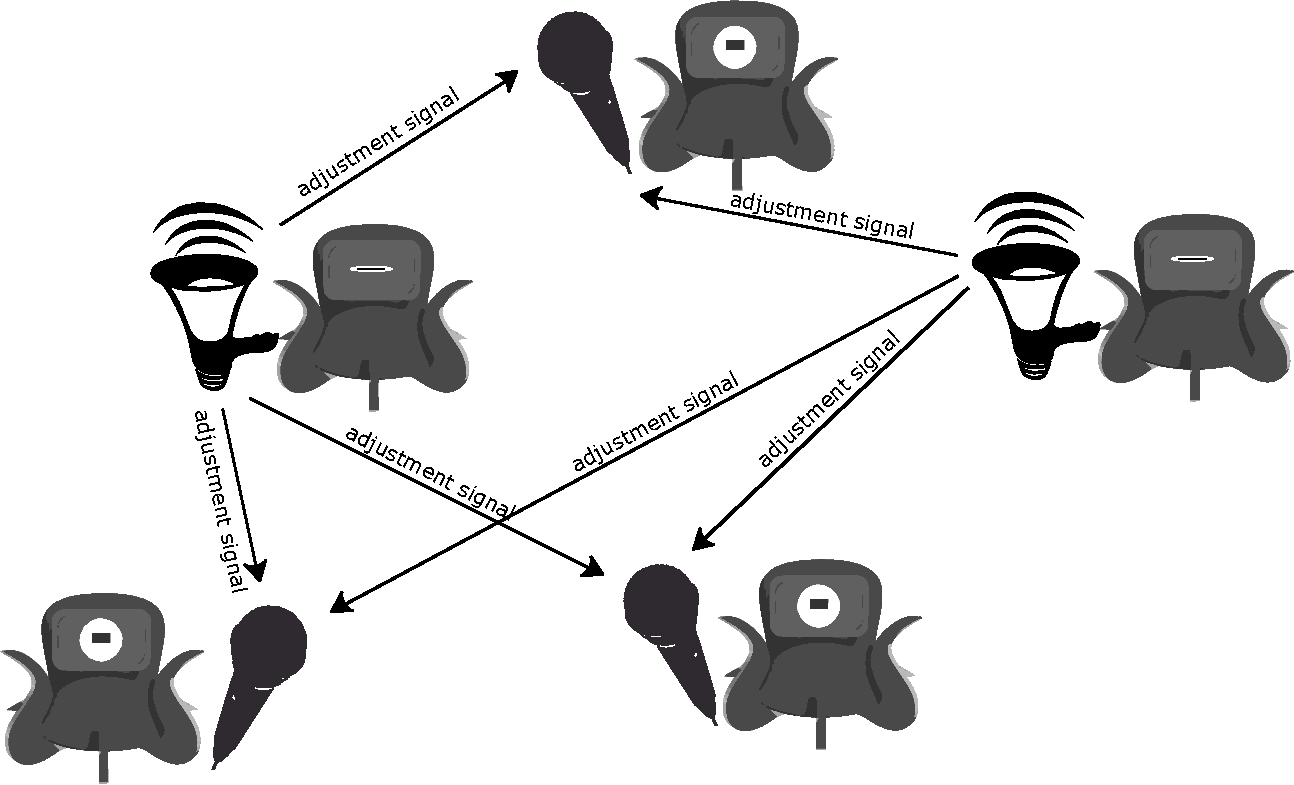
\includegraphics[width=0.9\linewidth]{Assets/DocSegments/Chapters/Implementation/Figures/Illustrations/schematic_initial_idea.pdf}
	\caption[Schema of the developed musical multi robot collective.]{Schema: the musical robot collective entraining to synchronize to each other, or more specifically to achieve harmonic synchronization, through performing phase \& frequency adjustments. Robots that are not firing at the moment will adjust themselves after hearing a transmitted ``fire'' / adjustment signal from a neighbouring firing robot.}
	\label{fig:first_idea:first_fig}
\end{figure}

Envision a decentralized (i.e. no central control) multi-agent collective scenario consisting of musical robots modelled as oscillators. These are solely communicating through brief ``fire''-like audio-signals—greatly inspired by Nymoen's synchronizing ``fireflies''. They are not initially synchronized in their firing of audio-signals; but as time goes, they are entraining to synchronize to each other by adjusting their phases and frequencies when/after hearing each other's audio-/fire signals. If they then, after some time of listening to each other and adjusting themselves accordingly, succeed in becoming synchronized — we then will eventually see ``fire''-events/-signals line up at an even underlying pulse or rhythm. Examples and demonstrations of this process are depicted in Figure \ref{fig:first_idea:first_fig} as well as in Figure \ref{fig:illustrative_developed_system} in Chapter \ref{chap:introduction}.

This chapter gives an overview of the developed musical multi-robot system\footnote{\url{https://github.com/theRealSherapat/CompSA} (accessed 2022.05.29)}, already existing methods implemented for it, as well as the performance measurement used to evaluate these methods with. The main goal of the implemented system is to allow for individual musical agents in a musical multi-agent collective to interact with each other, in order to achieve emergent and co-ordinating behaviour—in our case synchronization—with varying degrees of self-awareness, collective-sizes, and of difficulty and certainty in the environment and communication. More specifically, the goal with the design is to enable the robot collective to achieve so-called \textit{harmonic synchronization} (cf. \ref{sec:harmonic_synchrony}) within a relatively short time. Exactly what is meant by \textit{harmonic synchronization} will be expounded in Section \ref{sec:harmonic_synchrony}.

These goals firstly require of the agents the modelling of oscillators with their properties, like phase and frequency, as explained further in Subsection \ref{subsec:agent}. To allow for interaction and communication between the agents, mechanisms so that the agents can transmit ``fire'' signals, as well as listen for other agents's ``fire'' signals, is necessary as well, and is presented in Subsection \ref{subsec:fire_signal}.

Firstly, the newly developed synchrony simulator and its components will be presented and expounded in detail. Then, already existing methods implemented in the novel synchronization simulator for achieving the system target goal of \textit{harmonic synchrony} will be described. How the system target state of harmonic synchrony is detected in the synchronization simulator will then be described in Section \ref{sec:detecting_harmonic_synchrony}.



\section{Simulator setup: the musical multi-robot collective}
\label{sec:developed_system}

Unity\footnote{Unity Version 2021.2.0f1 is used in the developed simulator.} is originally a game development platform, but can also be used to create complex and interactive simulations. Apart from enabling the design, implementation, and testing of various synchronization paradigms and methods—the results of this synchronization can also be clearly and visibly be seen and heard, as showcased in the introductory Figure \ref{fig:illustrative_developed_system} as well as in the video link seen in the corresponding Figure caption.

	\subsection{The simulator environment and its hyperparameters}
	\label{sim_env_and_hyperparams}
	
	\begin{table}[ht]
		\centering
		\begin{tabular}{p{0.15\linewidth} | p{0.8\linewidth}}
		  \textit{\textbf{Notation}}  & \textit{\textbf{Definition}} \\ \hline
		  $r_i$ & Individual musical robot $i$. \\ \hline
		  $R$ & Musical robot collective consisting of all robots $r_i$. \\ \hline
		  $\phi_i$ & Phase of $r_i$'s oscillator component. \\ \hline
		  $\omega_i$ & Frequency of $r_i$'s oscillator component. \\ \hline
		  \textit{sim s} & Simulation seconds. The unit of measurement, w.r.t. to time, used in the thesis and simulation. Simulation time does not always correspond to real / physical time, depending on how fast the hardware is able to run the simulations.
		\end{tabular}
		\caption{Notation and terminology used throughout the thesis for system components.}
		\label{tab:synchrony_simulator_terminology}
	\end{table}
	
	
	\begin{table}[ht]
		\centering
		\begin{tabular}{p{0.25\linewidth} | p{0.7\linewidth}}
		  \textit{\textbf{Hyperparameter}}  & \textit{\textbf{Meaning}} \\ \hline
		  $|R|$ & Musical robot collective size, where R (as defined above) is the set of all musical robots $r_i$ , i = 1, 2, ... , $|R|$. \\ \hline
		  $Adj_{\phi}$ & The adjustment method, or update function if you will, used for synchronizing phases $\phi$. \\ \hline
		  $Adj_{\omega}$ & The adjustment method, or update function if you will, used for synchronizing frequencies $\omega$. \\ \hline
		  $t_{ref} $ & The time (sim s) robots are unresponsive to adjusting themselves (as a consequence of hearing other robots firing) directly after firing themselves. \\ \hline
		  $t_{ref}^{dyn}$ & Dynamic refractory period. Same as $t_{ref}$, only that now the refractory period is given as the percentage of robot $r_i$'s oscillator period (e.g. 10\% of $1/4Hz=0.25s$, i.e. $0.1*0.25s=25ms$, if the oscillator frequency $\omega_i=4Hz$). \\ \hline
		  $t_f$ & Legal firing time during which robots $r_i$ are allowed to fire when being detected harmonic synchrony for. Condition 5) harmonic synchrony detection requirement (cf. \ref{baseline:subsec:detecting_harmonic_sync} in Chapter \ref{chap:baseline}). \\ \hline
		  $k$ & Condition 6) harmonic synchrony detection requirement (cf. \ref{baseline:subsec:detecting_harmonic_sync} in Chapter \ref{chap:baseline}). \\ \hline
		  $t_{max}$ & Maximum time limit given to musical robot collectives during which the collective might achieve the target state of harmonic synchrony during, unless they are terminated and deemed ``synchronization fails.'' \\ \hline
		  $\omega_{min}^{init}$ & Minimum initial oscillator frequency a robot's frequency can be assigned at the start of simulations. \\ \hline
		  $\omega_{max}^{init}$ & Maximum initial oscillator frequency a robot's frequency can be assigned at the start of simulations.
		\end{tabular}
		\caption{The environmental and collective hyperparameters present and used for the synchronization simulator in Unity.}
		\label{tab:synchrony_simulator_hyperparameters}
	\end{table}
	
	\textbf{Hyperparameters further explained} \nl
	
	\textbf{$t_{ref}^{dyn}$}: Roboticists like e.g. K. Konishi and H. Kokame \cite{konishi_kokame} suggest that by reducing the time oscillators in wireless sensor networks are active (i.e. increasing inactive time), power usage can also be reduced—something which makes oscillator systems last longer as well as being better for the environment in the end. Hence, a as large $t_{ref}$ or $t_{ref}^{dyn}$ as possible, seems to have some real benefits in real systems.
	

	\subsection{The individual agent: a musical robot}
	\label{subsec:agent}

	As introduced and presented earlier in \ref{dr_squiggles}, our musical robot collective will then consist of models of M. J. Krzyzaniak and RITMO's \textit{Dr. Squiggles}.
	
	The aforementioned (cf. \ref{solojam_island}) 3D-models of these Dr. Squiggles robots for simulation are reused, with permission, for the simulation system designed in this thesis project. They can e.g. be seen in the introductory Figure \ref{fig:illustrative_developed_system}.

	Every musical robot or node have certain components, attributes, and characteristics that make it what it is. Such include an oscillator-component, consisting of the agent's oscillator-phase $\phi$ and oscillator-frequency $\omega$. Notions like ``agent'', ``robot'', ``firefly'', and ``oscillator'' will be used interchangeably throughout the thesis. The agents have an input-mechanism for hearing/detecting transmitted ``fire''-event signals from other agents, as well as an output-mechanism for transmitting or playing such ``fire''-/adjust-signals or tones, as is illustrated with the microphone and megaphone respectively in Figure \ref{fig:first_idea:first_fig}.
	
	\begin{table}[ht]
		\centering
		\begin{tabular}{p{0.25\linewidth} | p{0.7\linewidth}}
		  \textit{\textbf{Hyperparameter}}  & \textit{\textbf{Meaning}} \\ \hline
		  $\alpha$ & Phase coupling constant. The larger the $\alpha$, the more a robot adjusts its phase when hearing ``adjustment signals'' from neighbouring robots. \\ \hline
		  $Adj_\phi$ & Phase adjustment method used to synchronize phase values $\phi$ with. \\ \hline
		  $\beta$ & Frequency coupling constant. The higher the $\beta$, the more robots adjust their frequencies $\omega_i$. \\ \hline
		  $Adj_\omega$ & Frequency adjustment method used to synchronize frequency values $\omega$ with. \\ \hline
		  $m$ & Error memory length. The larger the $m$, the more error scores $\epsilon$ robots remember with which they use in their calculation of the self assessed sync score $s$. \\ \hline
		  $k_s$ & Integer number of nearest neighbour robots that are within a robot's self awareness scope, and hence telling how many neighbour robots a robot listens to for fire events. \\ \hline
		  $d_s$ & Physical radius (in Unity units) around a robot where robots closer to the robot than $d_s$ are within said robot's self awareness scope, and hence telling how far out from itself a robot listens for neighbours's fire events.
		\end{tabular}
		\caption{The hyperparameters possible to alter for the individual musical robots in the synchronization simulator in Unity.}
		\label{tab:synchrony_robot_hyperparameters}
	\end{table}
	
	In order to be able to analyse the musical scenario within which they are situated (self-assessment), as well as for adapting their musical output accordingly (self-adaptation), the agents are to some extent endowed with artificial intelligence and self-awareness capabilities. The robots are self-aware of their own phase and frequency, but are unaware of other agents's true phases and frequencies. They also possess the self-assessment capability of evaluating how much in- or out-of-synch they are, as seen in the greater context of the entire robot collective. When the agents hear the transmitted ``fire''-/adjust-signals, the agents are intelligent enough to adjust themselves in the direction of the system goal/target state.

	Unless otherwise is stated, the heterogenous visual looks of the Dr. Squiggles robots in Unity have no real difference in the simulator and is only that (for visual looks), not implying other values or methods used.

	
	\subsection{Robot communication: the ``fire''-signal}
	\label{subsec:fire_signal}
	
	Signals, in various forms, are omnipresent in our world, whether we notice it or not. They are used for guidance: e.g. traffic-lights send visual light-signals to drivers to ensure traffic-flow and collision-avoidance; sirens and alarms fire away with the loudest of audio-signals (sounds) so that its listeners will get out of harms way; our nerves send pain-signals through our nervous-system if we touch something burning hot to ensure we do not damage our hand severely. If you have ever tried to make a scary sound to scare away an animal—like a cat or crow—they might in fact flee from you if they think your audible signal was scary enough for them. In this specific case, for our musical robots in the musical synchronization simulator, signals will signify calls for adjustment (of oscillator phases $\phi$ and frequencies $\omega$ to be specific).

	These aforementioned audio-signals, also referred to as ``fire'' signals, ``flash''-signals, or adjust-signals, are transmitted whenever an agent's oscillator \textit{peaks} or \textit{climaxes} (i.e. after its cycle or period is finished, having phase $\phi(t)=1$) — or actually after every second \textit{peak}, as a way (discovered by K. Nymoen et al. \cite{nymoen_synch}) to attain the system target goal of \textit{harmonic synchrony}, to be elaborated upon in Section \ref{sec:harmonic_synchrony}.

	The ``fire'' signals are short and impulsive tones that the agents output through their loudspeakers. These short audio-signals/sounds ``wildly'' transmitted or played into the environment are then the only means of communication within the multi-agent collective, implying that are agents are pulse-coupled, not phase-coupled, oscillators. In other words, our agents will communicate and co-ordinate with each other through the very typical multi-agent system concept of \textit{stigmergy}.

	When an agent detects a ``fire''-/adjust-signal, the agent will adjust its own oscillator-properties (phase $\phi$ and frequency $\omega$), depending on which type of problem the agents are to solve. No individual agent is directly able to adjust or modify the state or properties of any other agent, only its own.
	
	% Exactly the type of problems we attempt to solve in this thesis will be presented now in Section \ref{sec:phase_methods} and Section \ref{sec:frequency_methods}.
	

		\subsubsection{Under the hood in the simulator}
		\label{SA_scopes_implemented}
		
		Three distinct \textit{self awareness scope} (cf. \textbf{Domain} in \ref{conceptual_SA_framework}) scenarios are implemented for each individual musical robot in Unity:
		
		\begin{enumerate}
			\item \textbf{$k_s$ nearest neighbours self awareness scope}: Each individual robot hears the $k_s$ nearest neighbouring robot's ``fire'' signals (cf. \ref{subsec:fire_signal}). In this scenario, at least for small $k_s$ values, robots can have more limited and local knowledge.
			\item \textbf{Radial $d_s$ self awareness scope}: Each individual robot hears neigbouring robots's ``fire'' signals within a radius $d_s$ around it. In this scenario, robots's self awareness scope is more focussed on the spatial locations of other robots, and can also simulate the robot only hearing robots close in space to itself.
			\item \textbf{Global self awareness scope}: Each individual robot hears all other neigbouring robots's ``fire'' signals. In this scenario, robots have maximum and global knowledge when it comes to awareness of other neighbouring robots.
		\end{enumerate}
		
		In this way, the degree to which robots are self aware of or communicating with other robots is increasing. The effects of increasing or decreasing this degree of self awareness are shown in Chapter \ref{chap:experiments_and_results}, and especially in \ref{exp:phasesync:increasing_SA_deg} and \ref{exp:phase_and_freq_sync:increasing_SA_deg}.
		

		\subsubsection{Audible to human simulator observer}
		\label{human_audible_fire_signals}

			\paragraph{Fire signal design}
			The fire signal audible to the human observer watching and listening to the musical robots synchronizing to each other should be distinct and short enough so that one can clearly distinguish between which robots are firing and when. At the same time, the firing-sounds should to the human observer not be too sharp and loud to listen to so that it is uncomfortable observing the musical robot collective. Keeping these aspects in mind, some relatively soft and pleasant firing-sounds from an instrument usually associated with harmonious music—the harp—were produced and developed for the synchronization simulator.
			
			Some manually and empirically perceived harmonious (in terms of sounding good when played together) musical tones were digitally reproduced and recorded in the form of harp plucks. This was achieved using the music-making system and digital synthesizer LMMS, and a digital string-instrument in the form of a LMMS-plugin from DSK Music\footnote{\url{https://www.dskmusic.com/dsk-world-stringz-updated/} (accessed 2022.05.17)}. The musical tones, perceived to be harmonious when being heard simultaneously and reproduced with the digital harp instrument, were some of the very first tones perceived in the intro of Pogo's song ``Strangerous\footnote{\url{https://www.youtube.com/watch?v=cRzcsXDBn8g} (accessed 2022.05.17)}.'' One possible avenue to explore in order to find harmonious chords or tones—when played together—in a more automatic approach, live and online during simulation, is discussed in Further work in Chapter \ref{chap:conclusions}.
			
			However, the harp-sounds produced with DSK's LMMS-plugin are primarily long and constant harp plucks, as shown in Figure \ref{fig:sub:harp_sound}. Using such harp plucks as a fire-sound directly can make it hard to distinguish to the human ear when multiple robots are playing these frequently and simultaneously. The harp-sounds thus need to be slightly edited—which they in our implementation were in the audio-editing program Audacity—so that the long and constant harp pluck became more of a ``quick'' and distinguishable (when played often by several agents) ``sound-bullet'' — essentially what we want in a solid ``fire'' signal sound. The ``before'' and ``after'' of such an audio-editing process is depicted in Figure \ref{fig:fire_signal_designing}. Edits performed on waveform \ref{fig:sub:harp_sound} to obtain waveform \ref{fig:sub:harp_fire_sound} consists of effects like ``Fade Out'', to dampen the sound in the tail of the waveform and get a shorter sustain as it is called, and hence obtaining a ``quicker'' sound. It also includes, in the complete beginning, the ``Amplify'' effect, in order to get a as high ``attack'' or maximum amplitude as wanted to make the fire-sound audible enough before it quickly decays. And lastly, obviously it was needed to cut the waveform accordingly, specifically from the time it had amplitude $\approx 0$ to the end of the waveform.

			\begin{figure}[ht!]
				\centering
					\begin{subfigure}[t]{\textwidth}
						\centering\captionsetup{width=.8\linewidth}%
						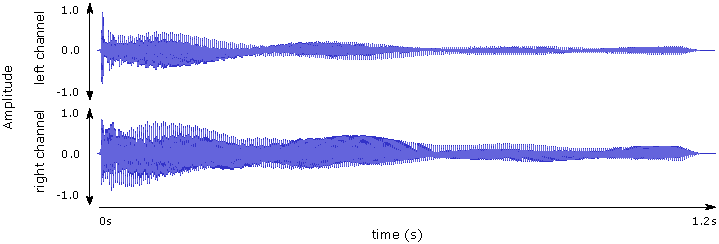
\includegraphics[width=\linewidth]{Assets/DocSegments/Chapters/Implementation/Figures/Illustrations/waveform_Strangerous_1_1.pdf}
						\caption{An unedited and pure harp sound (stereo audio waveform).}
						\label{fig:sub:harp_sound}
					\end{subfigure}
					%
					\begin{subfigure}[t]{\textwidth}
						\centering\captionsetup{width=.8\linewidth}%
						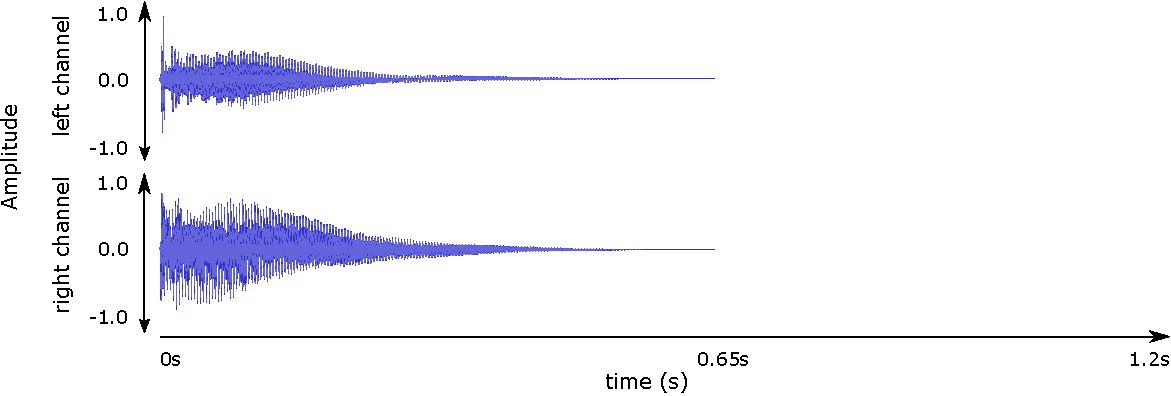
\includegraphics[width=\linewidth]{Assets/DocSegments/Chapters/Implementation/Figures/Illustrations/waveform_Strangerous_1_1_fire_signal.pdf}
						\caption{The pure harp sound from \ref{fig:sub:harp_sound} transformed into a fire signal.}
						\label{fig:sub:harp_fire_sound}
					\end{subfigure}
				\caption[Editing a longer and pure harp pluck to become a shorter fire signal.]{Here we see the starting point and end result of a fire sound design process, where the longer and pure harp sound in \ref{fig:sub:harp_sound} got edited and transformed into the more rapid fire sound in \ref{fig:sub:harp_fire_sound}.}
				\label{fig:fire_signal_designing}
			\end{figure}


			\paragraph{Frequency based fire-sound assignment}
			
			Given that our developed system is not simply a synchronization-system, which could have been implemented with simpler electrical circuits e.g. \cite{konishi_kokame}, but also a musical robot system — the display and expression of the robots synchronizing and becoming synchronized should have a musical dimension, as well as providing a clear way to see whether the robots are getting synchronized or not. Therefore, a musically interesting and meaningful way of signalizing the synchronization process was needed. The answers to the question of what is different between robots throughout the simulation plays a key part here; namely, e.g. the robot's oscillator frequencies. 
			Different musical tones were recorded (again with a harp instrument) and later edited into ``fire'' signals, as described above, with various signal lengths given their pitch.
			The idea was to assign, online and dynamically throughout the simulation run, ``fire''-signal-transformed musical tones with higher pitch (or waveform frequencies) to musical robots with the highest oscillator frequencies in the robot-collective. This is done by calculating a frequency percentage $\omega_\%$ a given robot $r_i$ has, as in the formula given in \ref{firesound_frequency} and visually in Figure \ref{fig:fire_signal_freq_assigning}.
			
			\begin{equation}\label{firesound_frequency}
				\omega_\% = \frac{\omega_i-\omega_0}{\omega_{max}-\omega_0},
			\end{equation}
	
			where $\omega_i$ is the oscillator frequency of robot $r_i$, $\omega_0$ is the fundamental or smallest oscillator frequency currently in the robot collective, and $\omega_{max}$ is the highest oscillator frequency currently in the robot collective.
			
			\begin{figure}[h]
				\centering
				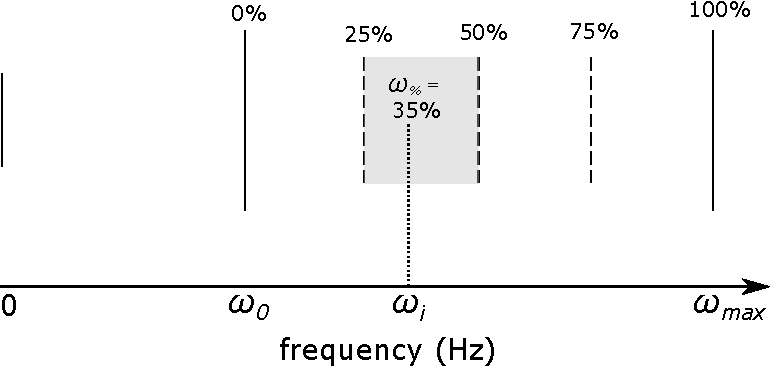
\includegraphics[width=0.7\linewidth]{Assets/DocSegments/Chapters/Implementation/Figures/Illustrations/frequency_firesignal_assigning.pdf}
				\caption[Schema of frequency based fire signal assignment.]{Schema of frequency based fire signal assignment in an example where four fire sounds with increasing frequency or pitch exist, and the robot is assigned the second lowest due to its oscillator frequency $\omega_i$.}
				\label{fig:fire_signal_freq_assigning}
			\end{figure}
			
			This percentage is then used in a manner like in the schema given in Figure \ref{fig:fire_signal_freq_assigning}, where the frequency percentage $\omega_\%$ is decides in which region, corresponding to a lower or higher pitch fire sound, the robot's frequency belongs to. Hence, robots are assigned fire sounds with higher pitch or frequency the higher frequencies the robots themselves have, and similarly fire sounds with lower pitch or frequency the lower oscillator frequencies the robots have.

		\subsubsection{Robot instansiation}
		
		Robots are spawned randomly in the Unity scene within a circle from origo until a certain radius according to the empirically found, through trial and error, formula for not too crowded robot collectives in \eqref{spawn_radius}.
		
		\begin{equation}\label{spawn_radius}
			radius_{spawn} = \frac{|R|}{6} \cdot r_{width} + 4,
		\end{equation}
		
		where $r_{width} = 5.7$ is the measured physical width or diameter in Unity of an individual robot $r$, and the term 4 simply is to add a bit more space to avoid crowding. The simple model was found through trial and error, and will make the robots spawn kind of like in a round pool of water.

% --- \section END. ---



\section{Synchronizing oscillator phases}
\label{sec:phase_methods}
	If we first assume constant and equal oscillator frequencies in our agents, we can take a look at how the agents adjust their initially random phases in order to synchronize to each other. Examples of how phase synchronization can look are given in Figure \ref{fig:strog_phase} and \ref{fig:nymoen_phase}. A more formal requirement and definition for phases to be deemed harmonically synchronized is also given below.
	
	For both of the implemented phase synchronization methods, Mirollo \& Strogatz and Nymoen's, the timing of when the update functions are used and applied is the same; Musical agents's phases get updated immediately as ``fire'' events from neighbouring robots are perceived. \nl
	
	\textbf{Legal phases definition:} \nl

	In an oscillator collective with heterogenous oscillator frequencies $\omega_i$, oscillator phases $\phi_i$ are harmonically synchronized when all oscillators's phase climaxes (i.e. $\phi=1$) or resets (i.e. $\phi=0$) occur exactly $T_{min} \cdot \mathbb{N}$ seconds later after $t_{synced}$, where $T_{min}=1/\omega_{max}$ for the highest oscillator frequency in the collective $\omega_{max}$, $t_{synced}$ is the time after the oscillator collective has become harmonically synchronized and the oscillator with the highest frequency $\omega_{max}$ has a phase climax or reset, and $\mathbb{N}$ are all natural (positive integer) numbers.
	
		\subsection{Implementing and verifying Mirollo-Strogatz's phase adjustment} % used '-adjustment' before
		
		Mirollo-Strogatz's approach for synchronizing phases in oscillators, as introduced in \ref{mirollo_strogatz_phase_adjust}, is implemented in the Unity simulator, and each agent is endowed with \textbf{phase update function \eqref{strog_phase}} with which they adjust themselves according to when perceiving a ``fire''-signal as described above.
		
		The verification that this works in the newly built synchronization simulator was performed by dumping all agents's phase values $\phi(t)$ during simulation runs. A plot of these $\phi(t)$-values, evolving through simulation time in seconds, is shown in Figure \ref{fig:strog_phase}.
		
		\begin{figure}[h]
			\centering
			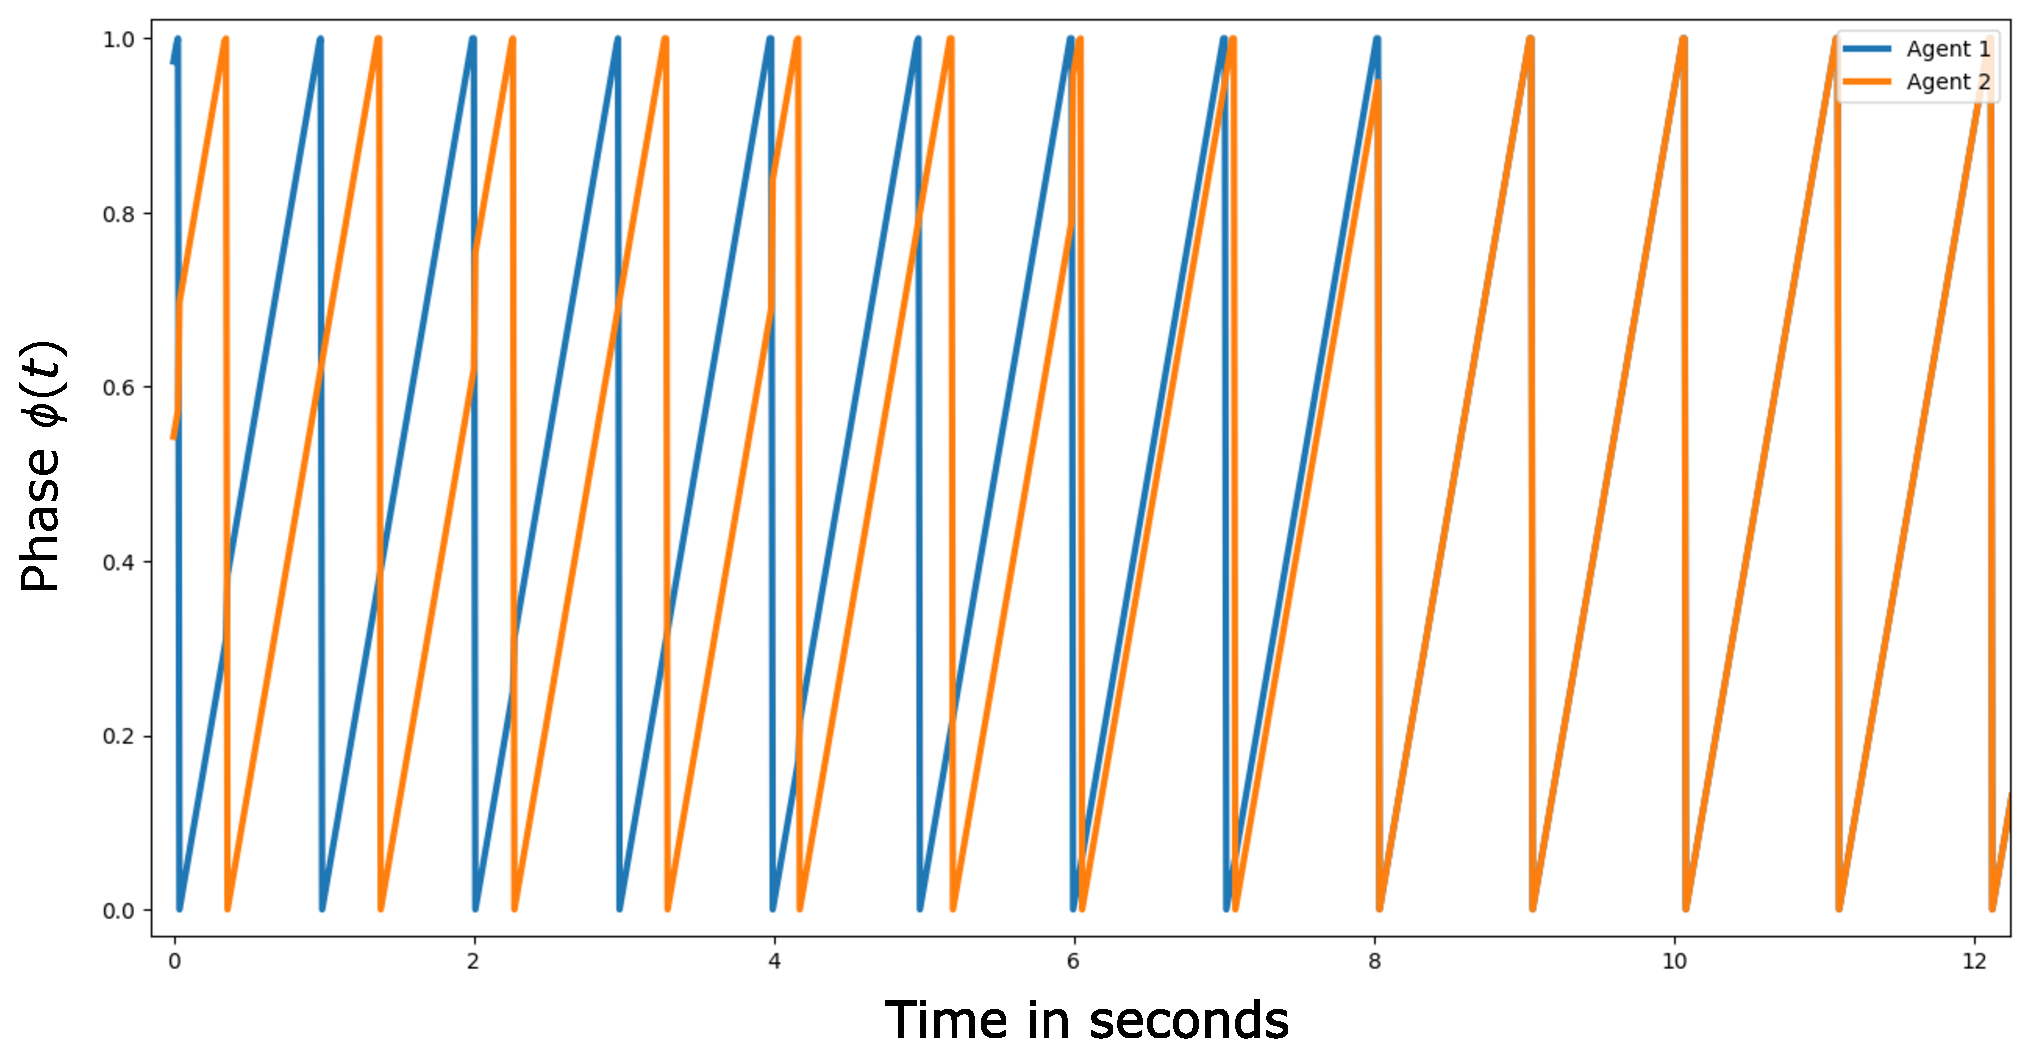
\includegraphics[width=0.9\linewidth]{Assets/DocSegments/Chapters/ExperimentsAndResults/Figures/Validations/MirolloStrogatzPhaseAdjustmentSecondTry.pdf}
			\caption[Illustration of Mirollo \& Strogatz's ``standard'' phase adjustment ($Adj_{\phi}$) method.]{``Standard'' phase adjustment with Mirollo-Strogatz's approach}
			\label{fig:strog_phase}
		\end{figure}
		
		
		\subsection{Implementing and verifying Nymoen's bi-directional phase adjustment} % used 'Shifts' before
		
		Nymoen's approach for synchronizing phases in oscillators, as introduced in Section \ref{subsec:nymoen_phase_adjust}, is implemented in Unity, and each agent is endowed with \textbf{phase update function \eqref{nymoen_phase}} with which they adjust themselves according to when perceiving a ``fire''-event as described above.
		
		The verification that this works in the newly set-up simulator-environment was performed by analysing carefully all the agents's phase values $\phi(t)$ throughout a simulation run. Such an analysis plot can be seen in Figure \ref{fig:nymoen_phase}.
		
		\begin{figure}[h]
			\centering
			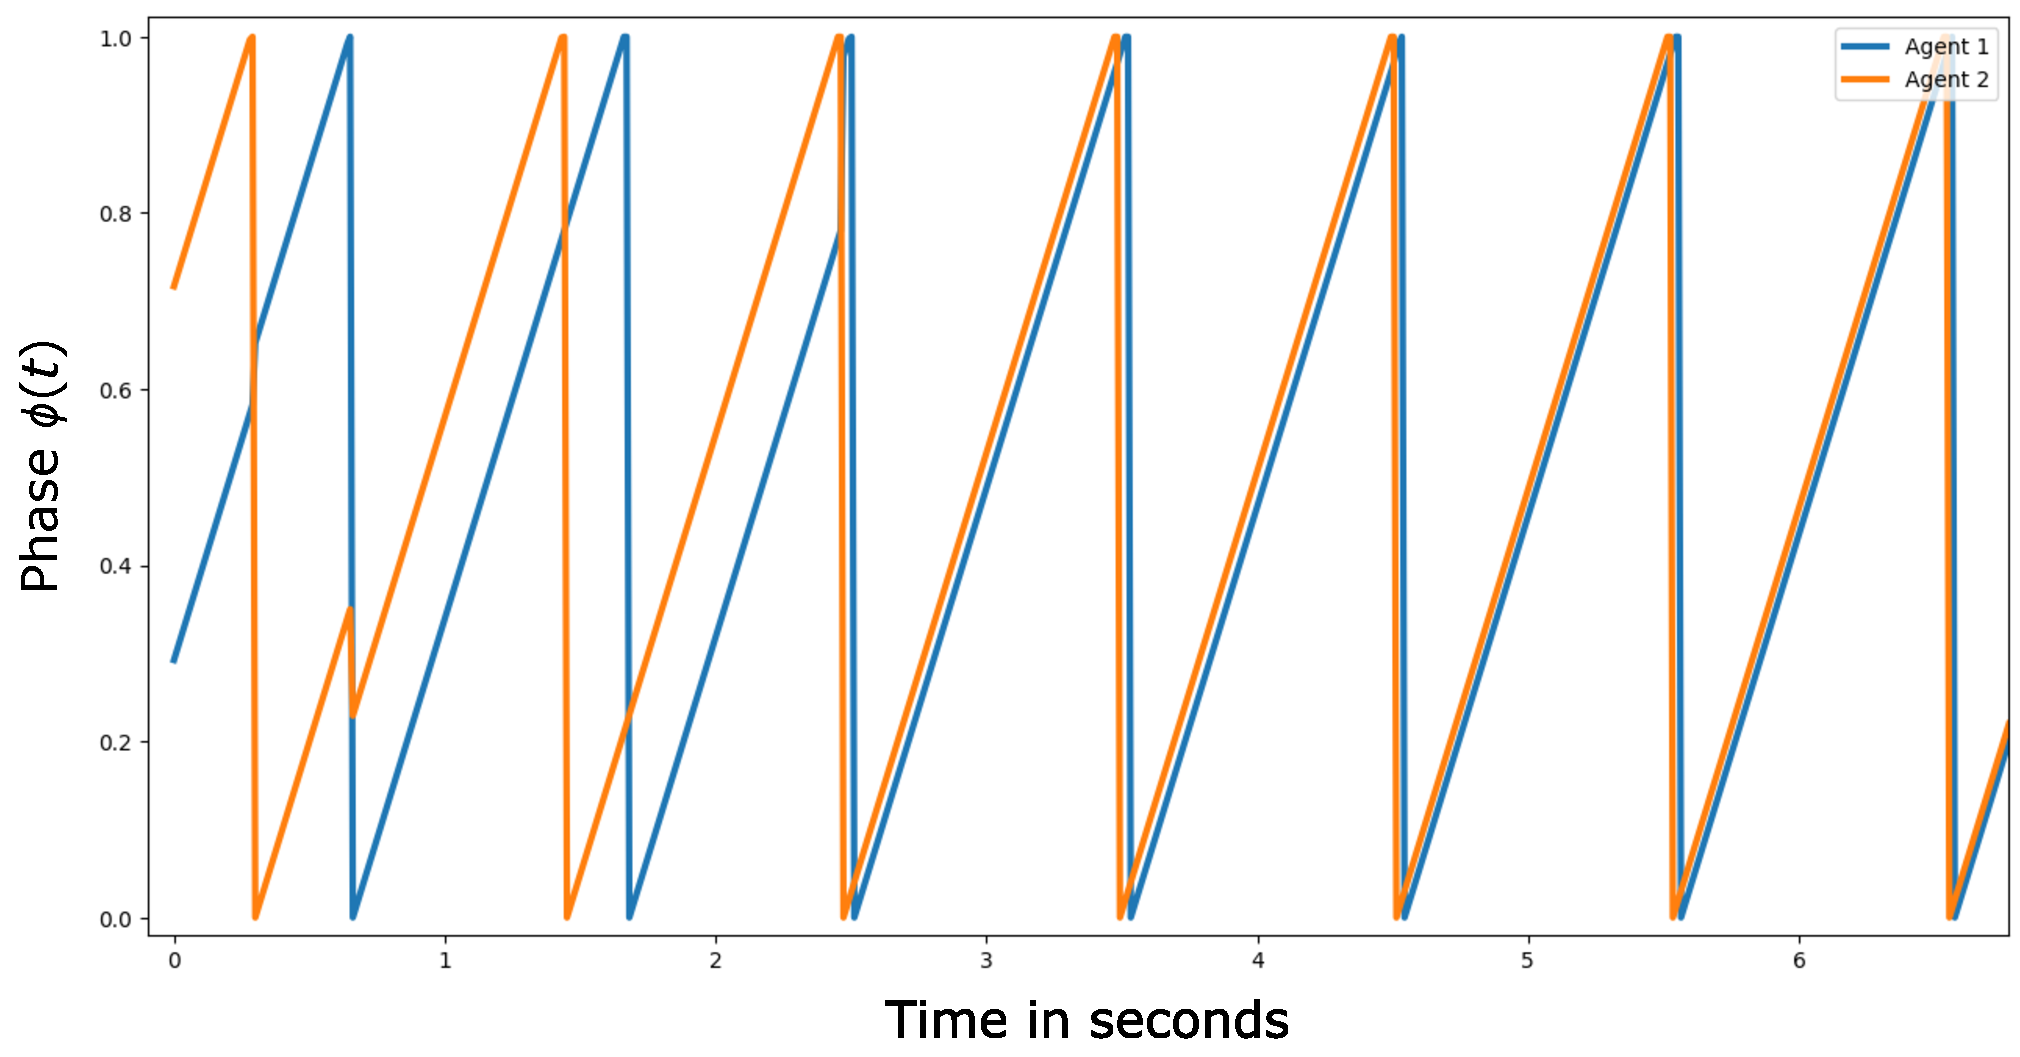
\includegraphics[width=0.9\linewidth]{Assets/DocSegments/Chapters/ExperimentsAndResults/Figures/Validations/KNymoenPhaseAdjustmentSecondTry.pdf}
			\caption[Illustration of Nymoen's bi-directional phase adjustment ($Adj_{\phi}$) method.]{Bi-directional phase-adjustment with Nymoen's approach}
			\label{fig:nymoen_phase}
		\end{figure}	
	
	
\section{Synchronizing oscillator frequencies}
\label{sec:frequency_methods}

	When we open up for the possibility for heterogenous frequencies in our musical agent collective, we open up to exciting musical aspects like the playing of diverse rhythmic patterns as e.g. mentioned in Section \ref{sec:harmonic_synchrony}, but we then also need to not only synchronize phases, but also frequencies, simultaneously. An example of how Nymoen's frequency synchronization, implemented in the current Unity synchronization simulator, can look like is given in Figure \ref{fig:frequency_synch}.
	
	For Nymoen's frequency synchronization method, the timing for when the update function is to be used and applied is a bit peculiar, and only happens once every phase climax ($\phi=1$). This is due to its utilization of the so-called reachback firefly algorithm, as explained in Subsection \ref{subsec:nymoen_freq_adj} and displayed in the corresponding Figure \ref{fig:nymoen_freq_adjust_illustration}.
	
	\begin{figure}
		\centering
		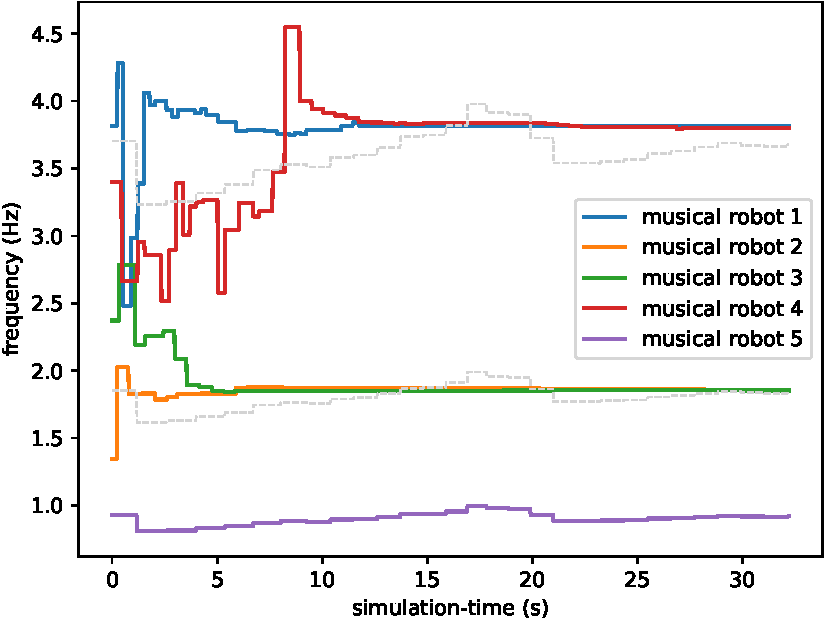
\includegraphics[width=\linewidth]{Assets/DocSegments/Chapters/ExperimentsAndResults/Figures/Explanations/FrequencySynchronizationPlot.pdf}
		\caption[Simulation run plot: frequency plot.]{Frequency synchronization for five robots in a Unity synchronization simulation run achieving harmonic synchrony after 30 seconds. Note how the legal harmonic frequencies (dashed gray lines) are defined by the lowest—fundamental—frequency $\omega_0$ in the robot collective fluctuating slightly below 1Hz, correctly leading to the legal frequencies right below 2 and 4 Hz.}
		\label{fig:frequency_synch}
	\end{figure}
	
	We hence now introduce randomly initialized, non-constant, and heterogenous oscillator frequencies in our musical agents. The agents are now required to synchronize their initially different and random frequencies, so that frequencies are ``legal'' and \textit{harmonically synchronized}. Such ``legal'' frequencies are now described clearly in detail. \nl
	
	\textbf{Legal frequencies definition:} \nl

	Building upon Nymoen's definition of harmonic synchronized oscillator frequencies (cf. \eqref{nymoen_legal_freqs}), a consise definition for the legal frequencies can be given as follows. All musical oscillators $i$, in a harmonically synchronized state, will have frequencies $\omega_i$ which are element in the mathematical set

	\begin{equation}\label{impl_legal_freqs}
	\Omega_{legal}(\omega_0) = \omega_{0} \cdot 2^{\mathbb{N}_0} = \{\omega_{0}, 2\omega_{0}, 4\omega_{0}, 8\omega_{0}, ...\} ,
	\end{equation}

	where $\omega_{0}$ is the lowest frequency in the oscillator collective (or the fundamental frequency if you will), and $\mathbb{N}_0$ are the natural numbers including the number zero. \nl

	If e.g. the smallest oscillator frequency in the musical oscillator collective ($\omega_0$) was equal to 1.5Hz, \textit{legal} frequencies the rest of the oscillators in the collective could have would be $\Omega_{legal}$(1.5Hz) = \{1.5Hz, 3Hz, 6Hz, 12Hz, ...\}.

	Hence, in terms of frequencies $\omega_i$ for all oscillators $i$ in the oscillator network, we have \textit{harmonically synchronized} and \textit{legal} oscillator frequencies $\omega_i$ if (and only if)

	\begin{equation}\label{synced_freqs}
	\omega_i \in \Omega_{legal}(\omega_0) , \forall i.
	\end{equation} \nl

	This state of \textit{harmonic synchrony} is then the system goal state K. Nymoen et al. achieve using their phase and frequency update functions, as explained in Sections \ref{sec:nymoen_phase_updates} and \ref{sec:nymoen_freq_updates}; and is also the target or goal state we want to continue achieving and experimenting for in this thesis.
	
	
	\textbf{Implementation details:} \nl
	
	In the newly proposed Unity simulator environment, the previously introduced self-assessed sync score $s(n)$ (in \ref{s_n}), encompassing the approach's main self awareness capabilities, is implemented as the median of a list containing \textit{m} error-scores $\epsilon$. Such an error score list of length $m$ is easily implemented by a list called \textit{errorBuffer}:
	
	\begin{equation}
	\label{error_buffer}
		errorBuffer = \{\epsilon(n), \epsilon(n-1), ... , \epsilon(n-m)\},
	\end{equation} \nl
	
	then leading to:
	
	\begin{equation}
	\label{self_assessed_synch}
		\begin{array}{rrclcl}
		s(n) & = & median(errorBuffer) \\ 
		& = & median(\{\epsilon(n), \epsilon(n-1), ... , \epsilon(n-m)\}) \in [0, 1],
		\end{array}
	\end{equation} \nl
	
	where $n$ is the latest observed ``fire-event'', and $m$ is the number of the last observed ``fire''-events we would like to take into account when calculating the self-assessed synch-score. \nl
	
	Regarding the ``frequency-update-contributions'' (the $H$-values described in \ref{H_n}) in my Unity-simulator, all the calculated H-values are accumulated and stored in an initially empty C\#-list (of floats), referred to as $H(n)$, at once they are calculated. The $H(n)$-list is then consecutively ``cleared out'' or ``flushed'' when its H-values have been used for the current period's frequency adjustment (i.e. at the phase climax, when $\phi(t)=1$), and is then ready to accumulate new H-values during the next period.
	
	By using K. Nymoen et al.'s frequency adjustment method, synchronization of initially random frequencies in our newly developed Unity simulator is achieved.
	
	The details of how the Dr. Squiggles in Unity adjust and eventually synchronize (harmonically) their oscillator frequencies, is shown in Algorithm \ref{AddNthFireEventsHToList} and \ref{RFAAdjustFrequency}. Algorithm \ref{AddNthFireEventsHToList} outlines how the ``frequency adjustment contributions'' $H$ get calculated as soon as the Dr. Squiggles hear a neighbour Dr. Squiggle sending a ``fire'' signal; whereas Algorithm \ref{RFAAdjustFrequency} shows how these previously calculated $H(n)$ values are used to obtain the new and updated oscillator frequency $\omega_i(t^+)$ with which individual oscillators assign their frequencies to after each phase climax (i.e. when $\phi=1$).
	
	\begin{algorithm}
	\caption{Calculating frequency update contributions $H$ for a robot}\label{AddNthFireEventsHToList}
	\begin{algorithmic}[1]
	\Procedure{}{$\phi(t), m$}
		\If {not in refractory period}
			\State $\epsilon \gets$ sin$(\pi \phi(t))^2$ \Comment{\tcol[gray]{Step 1}} % $n$th fire event's error score at time $t$
		\Else
			\State $\epsilon \gets 0$
		\EndIf
		\State $\epsilon$ is added to $errorBuffer$
		\State $s \gets$ median$\{\epsilon(n), \epsilon(n-1), ..., \epsilon(n-m)\}$ \Comment{\tcol[gray]{Step 2}}
		\State $\rho \gets -$sin$(2\pi\phi(t))$ \Comment{\tcol[gray]{Step 3}}
		\State $H \gets \rho \cdot s $ \Comment{\tcol[gray]{Step 4}}
		\State $H$ is added to list $H(n)$
	\EndProcedure
	\end{algorithmic}
	\end{algorithm}
	
	\begin{algorithm}
	\caption{Updating robot frequency with calculated $H$ contributions}\label{RFAAdjustFrequency}
	\begin{algorithmic}[1]
	\Procedure{}{$H(n), \beta$}
		\State $cycleHSum \gets 0$ \Comment{\tcol[gray]{Step 5 started}}
		\State $y \gets$ length$(H(n))$
		\ForAll {$ H \in H(n) $}
			\State $cycleHSum \gets cycleHSum + H$
		\EndFor
		\State $F(n) \gets 0$
		\If {$y$ not $0$}
			\State $F(n) \gets \beta \cdot cycleHSum / y$ \Comment{\tcol[gray]{Step 5 finished}}
		\EndIf
		\State Emptying $H(n)$ \Comment{\tcol[gray]{for new contributions next oscillator cycle}}
		\State $\omega_i(t^+) \gets \omega_i(t) \cdot 2^{F(n)}$
	\EndProcedure
	\end{algorithmic}
	\end{algorithm}
	
	

\section{Detecting harmonic synchrony}
\label{sec:detecting_harmonic_synchrony}

	The whole detection of harmonic synchrony in all its simplicity boils down to utilizing Unity's concept of Coroutines, meaning a process that can go on and be distributed across multiple frames in the simulator, as well as the firing of the robots as they every second phase climax ($\phi=1$) transmit a fire signal the simulator picks up on. As this in itself took several hundred lines of code\footnote{\url{https://github.com/theRealSherapat/CompSA} (accessed 2022.05.29)} to implement, the exact details of how it is implemented will not be expounded here.

	The performance measurement is used in the synchrony simulator to evaluate and test the multi-robot collective's ability to achieve harmonic synchronization. As mentioned in Subsection \ref{baseline:subsec:detecting_harmonic_sync}, K. Nymoen et al.'s requirements and illustrations (cf. Figure \ref{fig:nymoen_harm_sync_detect}) for achieving \textit{harmonic synchrony} serve as a blueprint or guide for how to similarly implement our synchrony or performance measurement. This performance measurement should be able, during synchronization simulation, to detect if harmonic synchronization has been achieved in our decentralized oscillator network. The successful triggering of this detection will then in turn terminate the synchronization simulation run and save to a dataset the time it took to synchronize (the performance score), in the case of a ``synchronization success.''

	The resulting and corresponding performance scores obtained using this performance measurement will then take values of the termination time (sim s) it takes for the robot collective, from the start of the synchronization simulation, to achieve the system target state of \textit{harmonic synchrony}, as specified in Section \ref{sec:harmonic_synchrony}.

	Now if \textbf{Conditions 5)-7)} from Subsection \ref{baseline:subsec:detecting_harmonic_sync} are kept and fulfilled, we have achieved harmonic synchrony.

	My specific implementation of the synchrony measurement essentially consists of enforcing all the requirements or rules listed in \ref{baseline:subsec:detecting_harmonic_sync}, given some constant $t_f$- and $k$-values (e.g. $80ms$ and $8$ respectively \cite{nymoen_synch}). And again—to recall from \ref{baseline:subsec:detecting_harmonic_sync}—$t_f$ is the short time-window within which nodes are allowed to fire at each beat, and $k$ represents how many times nodes have to fire at even underlying pulses/beats in a row without changing the $t_q$-period—before becoming harmonically synchronized.

	The requirement of firing evenly $k$ times in a row with identical $t_q$-periods can be—and in fact is in our implementation—enforced by incrementing an integer variable \textit{towards\_k\_counter} after a `legal' $t_f$-window has occured (i.e. one or more nodes fired inbetween the onset and ending of the $t_f$-window), and conversely by resetting \textit{towards\_k\_counter} to 0 when an illegally transmitted firing was heard during a `silent' (or so it was supposed to be at least) $t_q$-window, hence restarting the synchrony-detection process—as can be seen occuring several times in Figure \ref{fig:harmonic_synch_evolution}.
	
	\begin{figure}[h]
		\centering
		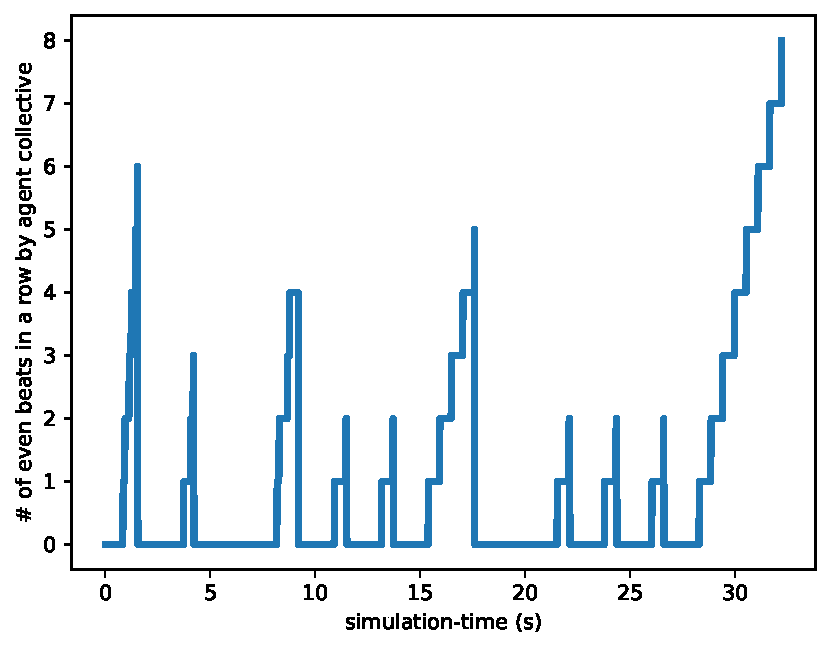
\includegraphics[width=0.85\linewidth]{Assets/DocSegments/Chapters/ExperimentsAndResults/Figures/Explanations/SynchronyEvolutionPlot.pdf}
		\caption[Simulation run plot: harmonic synchrony evolution plot.]{A \textbf{synchrony evolution plot}, displaying the temporal recording of the \textit{towards\_k\_counter} variable throughout a synchrony simulation run in Unity. The counter is incremented as the robot collective fires evenly within `legal' $t_f$ windows, and is conversely reset to 0 if illegal firings during `silent' $t_q$ windows are heard.}
		\label{fig:harmonic_synch_evolution}
	\end{figure}

	Note that in the specific simulation run in Figure \ref{fig:harmonic_synch_evolution}, the robots were on their way to achieve harmonic synchrony five times before the 10th second of the synchronization-simulation already, but since one or more of them fired `illegally' (i.e. inside a $t_q$-window), they were consequently `punished'—or rather deemed `not synchronized enough yet'—by getting their counter reset to 0. Eventually however, through further phase and frequency synchronization, the multi robot collective was in this case after 12.5 seconds able to achieve harmonic synchrony, when the ``even beat'' counter became equal to $k$, as well as all other requirements for achieving \textit{harmonic synchrony} was met. Note that this gives us a sense of how synchronized the robot collective is over time; the more even beats the robots have in a row, the closer they are to achieving harmonic synchrony.

	% Initially, the $t_q$-period/-window is not initialized, as it entirely depends on the frequencies to which the robot-collective converges to; however, when an illegal firing (i.e. a firing perceived during a $t_q$-window) occurs—$t_q$ is also then reset itself to a hopefully more correct value, given by the following formula:

	% \begin{equation}
	% \label{t_q_definition}
	% \begin{array}{rrclcl}
	% t_q^* & = & late\_t_q^*\_defining\_timevalue - early\_t_q^*\_defining\_timevalue - t_f \\
	% & = & median(t_1^`, t_2^`, ..., t_m^`) - median(t_1, t_2, ..., t_n) - t_f , \\
	% \end{array}
	% \end{equation}

	% where $n$ fire-events were recorded during the earlier $t_f$-window, and $m$ fire-events were recorded during the later $t_f$-window.
	
	If a certain amount of time, e.g. 5 simulation minutes \cite{nymoen_synch}, has gone without the detection of harmonic synchrony occuring, the simulation run is terminated as a ``fail''.


